Consider the following data: 

\begin{center}
    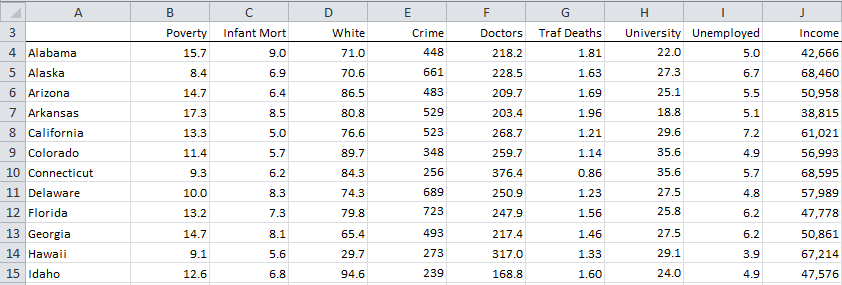
\includegraphics[width=0.9\textwidth]{img/e1p1.png}
\end{center}

Look over the data. By eye, which columns look correlated? Anticorrelated? Uncorrelated?

\begin{solution}
    A couple of examples are:
    \begin{itemize}
        \item Poverty is anticorrelated with income.
        \item Income is correlated with Doctors.
    \end{itemize}
\end{solution}
